\section{Testing the Demodulator}

The demodulation algorithm was tested by coding the algorithm in C.
The test app uses OpenGL and GLFW3 to provide a user interface and NVIDIA's
CUDA SDK to provide DSP power for the transform.

The software has a dependency on NVIDIA GPU cards.
The magic of GPUs lies in an architecture that efficently streams DRAM bursts
into and out of many CPU cores that operate in parallel.
The application operates on many values of R concurrently.
The development PC had a GTX 1080 graphics card.
Newer graphics cards such as the GTX 1660 ti offer nearly the same performance
at much lower cost: The DRAM bus isn't as wide but it uses a faster clock.
Look for a wide (such as 192-bit) memory bus and GDDR6.

With the GTX 1080, the CUDA-based algorithm was about 15 times as fast as an
FFTW-based version running on a single thread of a 3 GHz CPU core.
Running the algorithm in many threads on an expensive CPU could bring the
performance more in line with GPU performance,
but more likely is that memory bandwidth limitations will keep a CPU-based
solution slower than the GPU-based version.
Some of the higher end GPUs use stacked-die memory to provide much higher
bandwidth, so GPUs provide a real performance upgrade path.

The spectrogram consists of a range of R values spread vertically with time on
the horizontal axis.
Since the number of output points vary with R, time is normalized to the left 
edge of the image. At the left edge, the same amount of total time has elapsed
for each row of pixels.

\subsection{Spectrogram of a test chirp}

Figure \ref{fig:chirpTest1} shows a spectrogram image of a noisy
negative-chirp (R = -0.5) test signal with R on the vertical axis.
$R=-0.4$ is at the top and $R=-0.6$ is at the bottom.
A test signal was used to demonstrate detection of a chirp at
$R=-0.5$ and $N=4096$.
The chirp amplitude is 1/10 of the noise amplitude.
\begin{figure}
  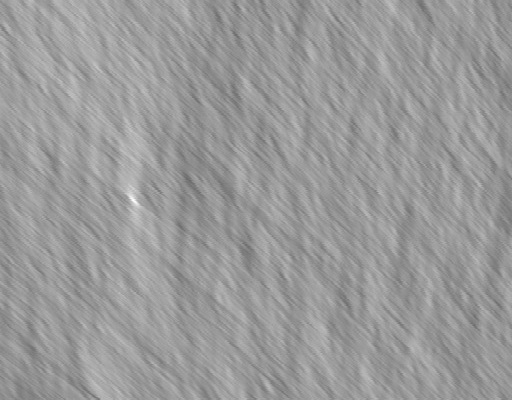
\includegraphics[width=\linewidth]{../source/chirp42m.jpg}
  \caption{Chirp power $(R<0)$ 20dB below noise.}
  \label{fig:chirpTest1}
\end{figure}

The noise produces a kind of slate or sandstone texture.
The white spot is the test chirp.
An oversample factor of 64 seems to be optimal.
Oversampling is the number of times an X input point is used in overlapping
operations. For example, 64 new input points for N = 4096.
Lower oversample factors leave more visible (patterned) artifacts.
Higher ones produce about the same smoothness with more computation load.
They don't really increase sensitivity.
Higher N mostly increases resolution and to some extent sensitivity.

White, pink, and brown noise (without the test chirp) has about the same 
appearance noted above.

\subsection{Spectrogram of music}

The first 2.5 minutes of Bach's Toccata and Fugue in D minor seemed like a good
test of tone-rich music. Organ notes are rich in harmonics.
The other test was the Surfaris ``Wipe Out'', another instrumental piece with
rich harmonics. Both were resampled to 22050 SPS.

\begin{figure}
  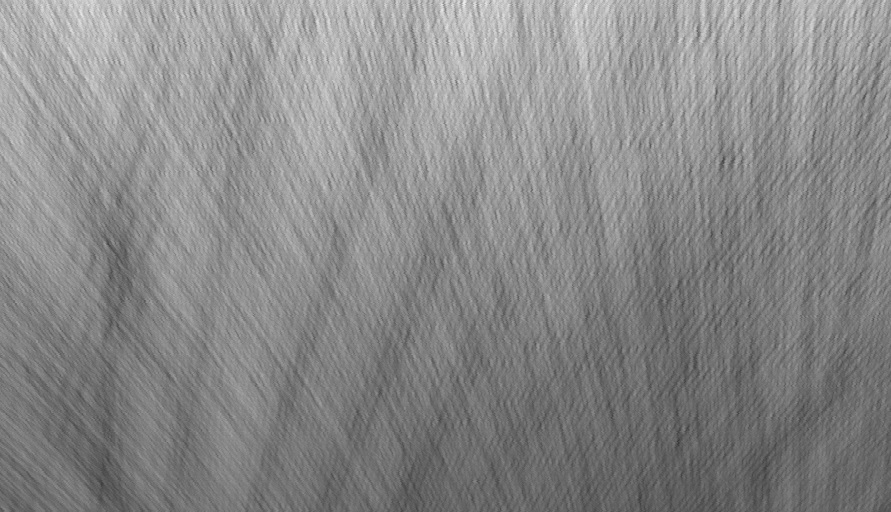
\includegraphics[width=\linewidth]{../source/bach220.jpg}
  \caption{Bach's Toccata and Fugue in D minor.}
  \label{fig:bach220}
\end{figure}

Figure \ref{fig:surfariswipeout} illustrates the texture of a periodic waveform.
Tones appear as wideband noise in the FFT output. 
They can produce wide but faint lines in the output.

\begin{figure}
  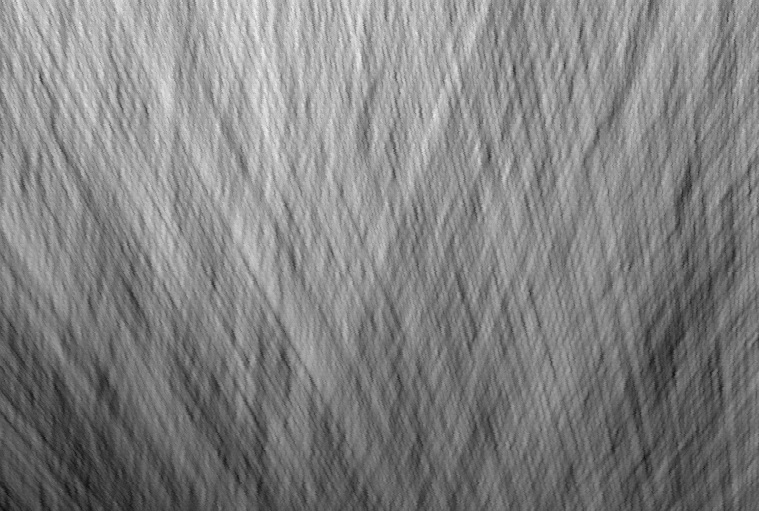
\includegraphics[width=\linewidth]{../source/surfariswipeout.jpg}
  \caption{The Surfaris Wipe Out.}
  \label{fig:surfariswipeout}
\end{figure}


\subsection{Spectrogram of an EEG signal}

EEG data was downloaded from the Sleep Spindles Database, excerpt 2.
Its web link is broken, but the data is in the wild.
Figure \ref{fig:excerpt2} shows the spectrogram during stage 2 sleep.

The spectrogram looks different from synthetic noise. 
It has the slate-like texture of synthetic noise but with ``scratches'' and ``hair''
that give a different appearance.

\begin{figure}
  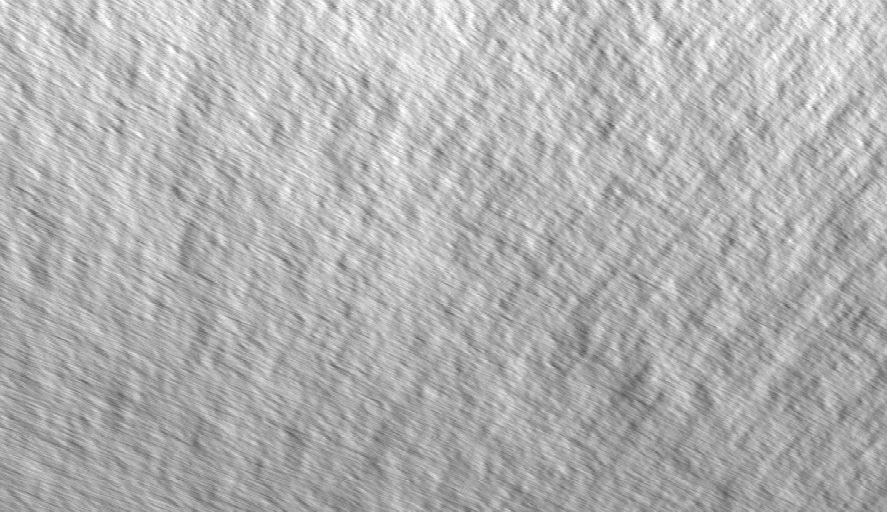
\includegraphics[width=\linewidth]{../source/excerpt2.jpg}
  \caption{EEG of a test subject in stage 2 sleep.}
  \label{fig:excerpt2}
\end{figure}

\begin{figure}
  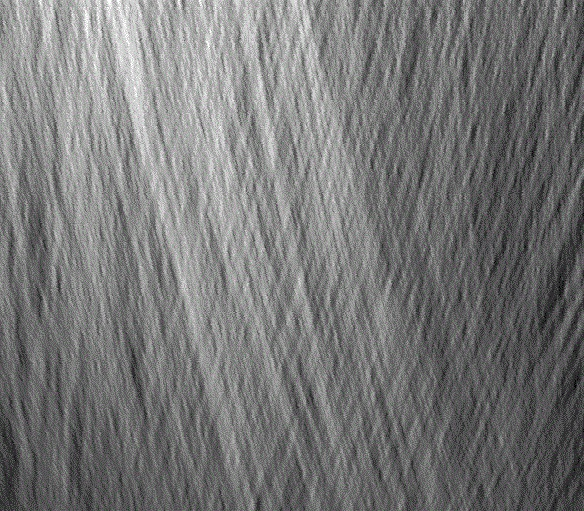
\includegraphics[width=\linewidth]{../source/wokessd.jpg}
  \caption{EEG of a test subject waking up from sleep for about 30 seconds.}
  \label{fig:wokessd}
\end{figure}

Although visual interpretation at this point is like reading tea leaves,
a trend that seems to be at play is that the warp factor, $\omega$, is not
constant. It changes exponentially, forming sloped (but mostly straight) lines
in the output.
These lines overlap in time and have different slopes.
Sometimes the slope shifts from positive to negative, through vertical.
Sometimes it seems a line with a slope will have a line near it with the
sign of its slope flipped.

The exponential emergent time model is much more complex than initially thought.
You would think we were dealing with nature.
The signals we're looking at aren't self-similar fractals.
The most computationally feasible means of decoding is probably to stick with
the exponential chirp transform model and post-process the 2D spectral image.
The transform depends on self-similarity in the time warping, which seems to
limit it to a power function. 

Rather than ``fix`` the transform, it should be easier to 
look for lines in the spectrogram.
It may be useful to keep in mind that an FM-modulated signal will produce
multiple parallel lines. The intensity of the lines would be reminiscent
of the frequency spectrum of a typical FM signal.
